\renewcommand{\MayorVer}{1}
\renewcommand{\MenorVer}{0}
\renewcommand{\Codigo}{G-1-PRO}
\renewcommand{\FechaPub}{2023--01}
\renewcommand{\Titulo}{Programa de verificación y actualización de información documentada}

\section{\Titulo}
\label{informacion.actualizacion}

\subsection{Objetivos}
\begin{itemize}
    \item \textbf{Establecer} un programa para la validación de la información documentada que maneja \GLS{RDF};
    \item \textbf{Procurar} que se validen los requisitos de cada programa establecido y con base en los nuevos requerimientos, se actualicen los mismos;
    \item \textbf{Proponer} fechas para la actualización de revisiones mayores y menores.
\end{itemize}

\subsection{Alcance}
\begin{itemize}
    \item Éste procedimiento va dirigido al área operativa encargada de la modificación de la información documentada y de los \gls{PPR} y \gls{PPRO} establecidos por \GLS{RDF};
    \item el alcance de la validación y revisión de la información contempla pero no está limitada a:
          \begin{itemize}
              \item comunicaciónes externas o internas;
              \item especificación de servicios;
              \item formularios;
              \item listas de verificación;
              \item listas;
              \item mapas de proceso;
              \item organigramas;
              \item planes;
              \item políticas;
              \item procedimientos;
              \item instrucciones de trabajo;
              \item programas.
          \end{itemize}
\end{itemize}

\subsection{Terminología y definiciones}
\begin{description}
    \defglo{PPR}
    \defglo{PPRO}
    \defglo{validacion-documental}
    \defglo{revision-documental}
\end{description}

\subsection{Procedimiento}

\begin{figure}[h]
    \centering
    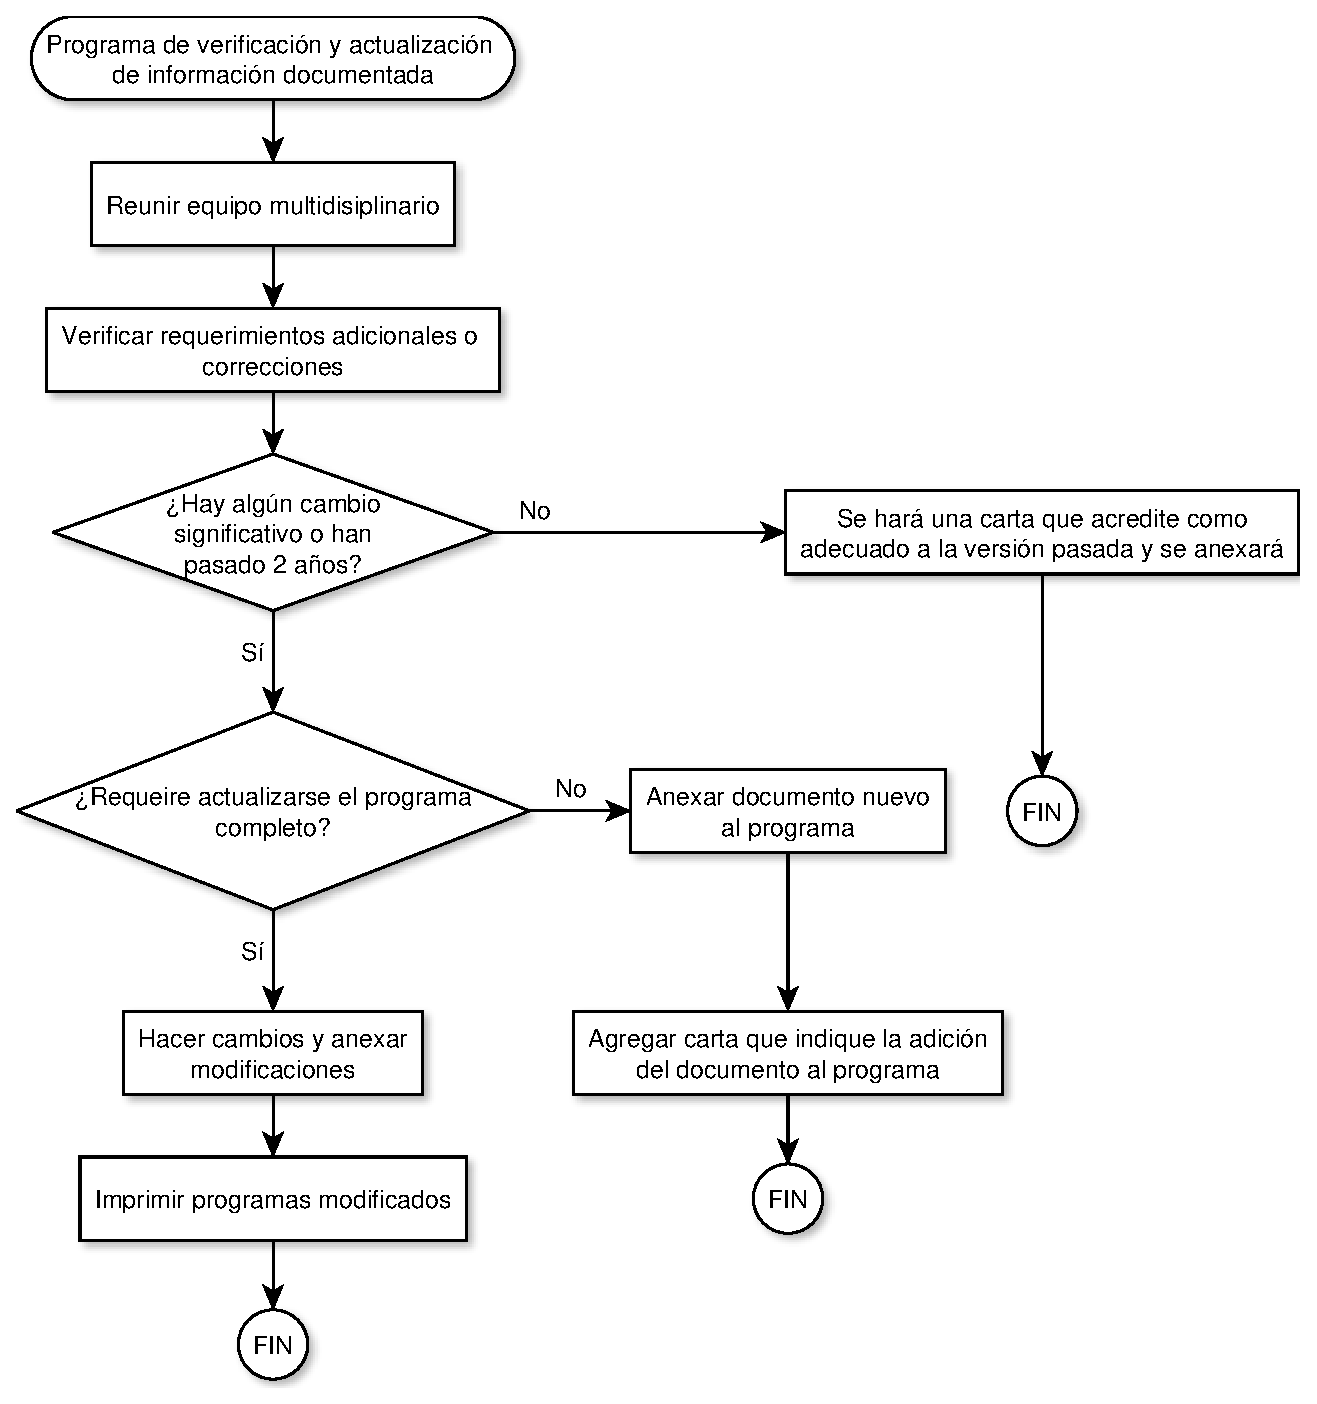
\includegraphics[width=0.5\linewidth]{src/diagramas/G1_AV1.eps}
    \caption{Diagrama de flujo del proceso para verificar y/o actualizar información documentada.}
\end{figure}

\subsubsection{Validación de la información documentada}
Se tienen que evaluar anaulmente los programas de \GLS{RDF} con el propósito de determinar áreas de oportunidad. Esto tiene que hacerse con ayuda de un equpo multidisciplinar constituido por administradores de las áreas operativas pertinentes a la información documentada que se va a validar.
\newpage

\subsection{Frecuencia}


% \vfill
% \begin{center}
%     \noindent\begin{tabular}{@{}>{\centering}p{2.5in}>{\centering}p{2.5in}@{}}
%         \small
%         \dotfill & \dotfill \tabularnewline
%         \textbf{\textit{Nombre del PCPC o visitante \\y empresa en que labora}}      & \textbf{\textit{Firma}}\\
%     \end{tabular}
% \end{center}
% \vfill

\begin{itemize}
    \item Se llevará a cabo una inspección por el personal de operaciones y en caso de ser observada una insatisfacción, se le pedirá al personal o visitante que incumplió con el reglamento cumplir con el requisito;
    \item El personal de calidad hará una inspección diaria de forma aleatoria y marcará en el formulario correspondiente si se cumple con el reglamento de ingreso de almacén.
    \item Si la desviación se repite frecuentemente se dará curso de capacitación al personal por parte de personal de calidad;
    \item Si después de haber capacitado al personal de almacén se siguen presentando desviaciones por causas injustificadas, será acreedor de una amonestación el personal interno que incumplió con el reglamento interno.
\end{itemize}


\begin{changelog}[simple, sectioncmd=\subsection*,label=changelog-1.0]
    \begin{version}[v=1.0, date=2023--01, author=Pablo E. Alanis]
        \item Primera edición.
    \end{version}
\end{changelog}